\section{Μηχανική Μάθηση}

Η ιδέα πίσω από τη μάθηση είναι ότι οι αισθήσεις δεν πρέπει να χρησιμοποιούνται απλώς για άμεση δράση, αλλά και για τη βελτίωση της ικανότητας ενός πράκτορα να ενεργεί στο μέλλον. Πράκτορας είναι οτιδήποτε μπορεί να θεωρηθεί ότι αντιλαμβάνεται το περιβάλλον του μέσω αισθητήρων, και επενεργεί σε αυτό το περιβάλλον μέσω μηχανισμών δράσης (Σχήμα \ref{fig:agent_environment_interaction}). Η μάθηση μπορεί να κυμαίνεται από την απλή απομνημόνευση των εμπειριών, μέχρι τη δημιουργία ολόκληρων επιστημονικών θεωριών. Εδώ περιγράφεται η επαγωγική μάθηση, κατά την οποία ένα σύστημα βελτιώνεται μέσω παρατηρήσεων \cite{Russell1994ArtificialIA}.

\begin{figure}[h]
  \centering
  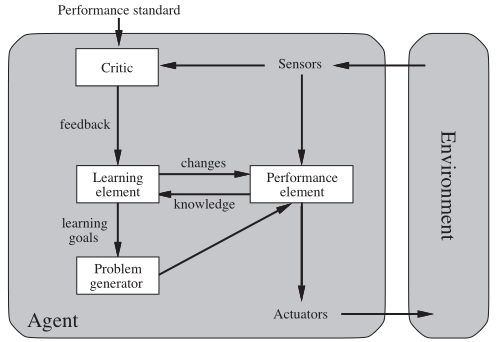
\includegraphics[width=\textwidth]{images/agent_environment_interaction.png}
  \caption{Αλληλεπίδραση πράκτορα με το περιβάλλον του}
  \label{fig:agent_environment_interaction}
\end{figure}

Ένας πράκτορας μπορεί να θεωρηθεί ότι περιλαμβάνει ένα στοιχείο εκτέλεσης, το οποίο αποφασίζει τι ενέργειες θα πραγματοποιήσει, και ένα στοιχείο μάθησης που τροποποιεί το στοιχείο εκτέλεσης έτσι ώστε να λαμβάνει καλύτερες αποφάσεις. Οι ερευνητές της μηχανικής μάθησης έχουν ανακαλύψει μια μεγάλη ποικιλία στοιχείων μάθησης. Για να γίνουν αυτά κατανοητά, είναι χρήσιμο να αποσαφηνιστεί το με ποιον τρόπο η σχεδίασή τους επηρεάζεται από το περιβάλλον στο οποίο θα εφαρμοστούν. Η σχεδίαση ενός στοιχείου μάθησης επηρεάζεται από τρία κύρια ζητήματα:
\begin{itemize}
    \item Ποιες συνιστώσες του στοιχείου εκτέλεσης πρέπει να μαθευτούν.
    \item Τι ανάδραση διατίθεται για τη μάθηση αυτών των συνιστωσών.
    \item Ποια αναπαράσταση χρησιμοποιείται για τις συνιστώσες.
\end{itemize}{}

Συνοπτικά \textbf{στοιχείο εκτέλεσης} είναι το στοιχείο του πράκτορα που είναι υπεύθυνο για εξωτερικές πράξεις και \textbf{στοιχείο μάθησης} το στοιχείο που είναι υπεύθυνο για την υλοποίηση βελτιώσεων στο σύστημα.

Ο \textit{τύπος της ανάδρασης} που διατίθεται για τη μάθηση είναι συνήθως ο πιο σημαντικός παράγοντας για τον προσδιορισμό της φύσης του μαθησιακού προβλήματος. Διακρίνονται τρεις περιπτώσεις: \textbf{μη επιβλεπόμενη μάθηση} (unsupervised learning), \textbf{επιβλεπόμενη μάθηση} (supervised learning) και \textbf{ενισχυτική μάθηση} (reinforcement learning).

\subsection{Μη επιβλεπόμενη μάθηση}
Το πρόβλημα της μη επιβλεπόμενης μάθησης περιλαμβάνει τη μάθηση προτύπων εισόδου χωρίς να παρέχονται συγκεκριμένες τιμές εξόδου. Δύο βασικές μέθοδοι είναι η \textit{ανάλυση σε κύριες συνιστώσες} (Principal Component Analysis - PCA) και η \textit{ανάλυση συστάδων} (cluster analysis). Χρησιμοποιείται ευρέως στην εκτίμηση πυκνοτήτων πιθανοτήτων (pdf) στη στατιστική.

\subsection{Ενισχυτική μάθηση}
Η ενισχυτική μάθηση είναι ένα πεδίο της μηχανικής μάθησης που ασχολείται με τον τρόπο που πράκτορες λογισμικού πρέπει να πάρουν αποφάσεις και να τις εκτελέσουν σε ένα περιβάλλον ώστε να μεγιστοποιήσουν κάποια ανταμοιβή. Όπως και η μη επιβλεπόμενη μάθηση, δεν χρειάζεται συγκεκριμένες τιμές εξόδου. Υλοποιείται τυπικά με την μορφή αλυσίδων αποφάσεων Markov

\subsection{Επιβλεπόμενη μάθηση}
H επιβλεπόμενη μάθηση είναι η διαδικασία της χαρτογράφησης μιας εισόδου σε μία έξοδο, με βάση \textit{labeled} δεδομένων εισόδου, που αποτελούνται από παραδείγματα εισόδου-εξόδου. Με αυτόν τον τρόπο, εκτιμάται μια συνάρτηση με βάση αυτά τα ζεύγη παραδειγμάτων. Κάθε παράδειγμα, είναι ένα ζεύγος, που αποτελείται από ένα αντικείμενο εισόδου, τυπικά ένα διάνυσμα, και μια επιθυμητή τιμή εξόδου. Σε ένα ιδανικό σενάριο, ο αλγόριθμος θα μπορεί να εκτιμήσει σωστά την επιθυμητή έξοδο από περιπτώσεις που δεν έχουν χρησιμοποιηθεί κατά την εκπαίδευση. Σε αυτή την κατηγορία αλγορίθμων μάθησης, εντάσσονται και τα Νευρωνικά Δίκτυα που θα απασχολήσουν αυτή την εργασία.

Πιο αυστηρά, ο στόχος της επιβλεπόμενης μάθησης είναι: Δοθέντος ενός \textbf{συνόλου εκπαίδευσης} Ν παραδειγμάτων ζευγών εισόδου-εξόδου: $$(x_1,y_1), (x_2,y_2), ... (x_N,y_N)$$ όπου κάθε $y_i$ δημιουργείται από μια άγνωστη συνάρτηση $y=f(x)$, να βρεθεί μια συνάρτηση $h$ που προσεγγίζει την $f$.

Όταν η έξοδος $y$ ανήκει σε ένα σύνολο πεπερασμένων τιμών, (λ.χ. ναι, όχι, ίσως) το πρόβλημα μάθησης λέγεται \textbf{ταξινόμηση} (classification). Όταν το $y$ είναι ένας πραγματικός αριθμός, το πρόβλημα λέγεται \textbf{regression}.

\begin{figure}[h]
  \centering
  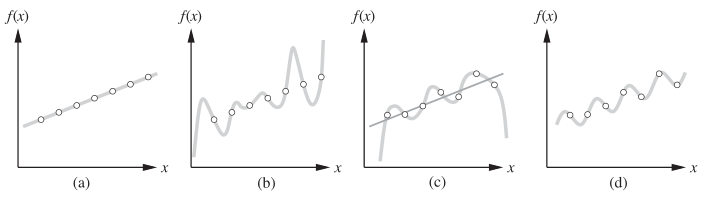
\includegraphics[width=\textwidth]{images/supervised_example_linear.png}
  \caption{Παραδείγματα ζευγών $(x,f(x))$ και υποθέσεις διαφορετικών βαθμών πολυωνύμου (a) 1ου βαθμού, (b) 7ου βαθμού. (c) Ένα διαφορετικό dataset και μια γραμμική εκτίμηση, (d) ημιτονοειδής εκτίμηση}
  \label{fig:supervised_example_linear}
\end{figure}

Στο Σχήμα \ref{fig:supervised_example_linear} φαίνεται ένα σύνηθες παράδειγμα, η προσαρμογή μιας καμπύλης σε ένα σύνολο ζευγών σημείων. Δεν είναι γνωστό ποια είναι η $f$ αλλά προσεγγίζεται με μια \textit{h} επιλεγμένη από τον χώρο υποθέσεων $\mathcal{H}$. Στο παράδειγμα αυτό είναι ένα σύνολο πολυωνύμων. 

Η επιβλεπόμενη μάθηση μπορεί να υλοποιηθεί επιλέγοντας την υπόθεση $h^*$ που είναι πιθανότερη με βάση τα δεδομένα:
\begin{CEquation}
\begin{split}
     h^* = \argmaxF_{h\subset\mathcal{H}} P(h|data)
     \label{eq:hypothesis_star}
\end{split}
\end{CEquation}


Η Εξίσωση \ref{eq:hypothesis_star} με βάση τον κανόνα του Bayes, μετασχηματίζεται στην Εξίσωση \ref{eq:hypothesis_star_bayes} και μπορεί κανείς να ισχυριστεί πως η εκ των προτέρων πιθανότητα $P(h)$ είναι μεγάλη για ένα πολυώνυμο μικρού βαθμού και χαμηλότερη για ένα πολυώνυμο μεγάλου βαθμού. Γενικότερα επιτρέπονται περίπλοκες ή \textit{παράξενες} προσεγγίσεις μόνο όταν κρίνεται ότι το απαιτούν τα δεδομένα, αλλά αποφεύγεται με τον να τους ανατίθεται χαμηλή πιθανότητα. Γενικά, αξίζει να σημειωθεί πως υπάρχει πάντα ένα tradeoff μεταξύ της εκφραστικότητας ενός χώρου υποθέσεων, και της πολυπλοκότητας της εύρεσης μιας καλής υπόθεσης μέσα σε αυτό το χώρο.

\begin{CEquation}
\begin{split}
     h^* = \argmaxF_{h\subset\mathcal{H}} P(data|h)P(h)
     \label{eq:hypothesis_star_bayes}
\end{split}
\end{CEquation}

\section{Νευρωνικά Δίκτυα}

Νευρωνικά Δίκτυα, ή με τον πιο δόκιμο όρο, Τεχνητά Νευρωνικά Δίκτυα (Artificial Neural Networks - ANN), είναι ένα σύνολο από τεχνητούς νευρώνες ή κόμβους \cite{Hopfield_1982}. Ουσιαστικά είναι υπολογιστικά συστήματα εμπνευσμένα από βιολογικά νευρωνικά δίκτυα που έχουν μελετηθεί σε εγκεφάλους διαφόρων ζώων \cite{Chen_2019}. Τα συστήματα αυτά 'μαθαίνουν' να εκτελούν συγκεκριμένο έργο λαμβάνοντας υπόψιν τους παραδείγματα, συνήθως χωρίς να είναι προγραμματισμένα με συγκεκριμένους κανόνες που αφορούν το εν λόγω έργο. Εκτελούν το έργο που τους ανατίθεται, χωρίς να έχουν πρότερη γνώση επί αυτού. 

\subsection{Νευρώνες} 

Ένα ANN βασίζεται σε μια συλλογή νευρώνων οι οποίοι μοντελοποιούν τους νευρώνες ενός βιολογικού εγκεφάλου. Κάθε σύνδεση, όπως οι συνάψεις στον εγκέφαλο, μπορεί να μεταδόσει σήματα στους άλλους νευρώνες. Ένας τεχνητός νευρώνας δέχεται το σήμα, το επεξεργάζεται και στη συνέχεια μεταβιβάζει το επεξεργασμένο σήμα στους νευρώνες με τους οποίους συνδέεται.

Αυστηρότερα, ένας νευρώνας είναι μια \textit{συνάρτηση}, και αποτελεί το δομικό στοιχείο ενός ANN. Δέχεται μία ή περισσότερες εισόδους, (που αντιπροσωπεύουν τα διεγερτικά μετασυναπτικά δυναμικά και τα ανασταλτικά μετασυναπτικά δυναμικά στους δενδρίτες των νευρώνων) τις προσθέτει και μεταδίδει μια έξοδο, (ή ενεργοποίηση που αντιπροσωπεύει το δυναμικό δράσης ενός βιολογικού νευρώνα που μεταδίδεται κατά μήκος του άξονά του). Η αντιστοίχηση φαίνεται στο Σχήμα \ref{fig:biological_neuron_artificial_neuron_cmp}. Συνήθως σε κάθε είσοδο ανατίθεται ένα βάρος και το άθροισμά τους δίνεται ως είσοδος σε μια μη γραμμική συνάρτηση που αποκαλείται \textbf{\textit{συνάρτηση ενεργοποίησης}} ή \textit{συνάρτηση μεταφοράς} του νευρώνα.

\begin{figure}[h]
  \centering
  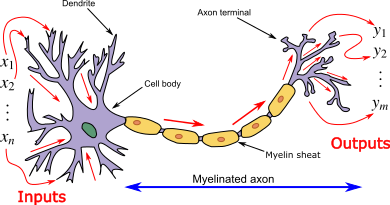
\includegraphics[width=\textwidth]{images/Neuron3.png}
  \caption{Νευρώνας και μυελινωμένος άξονας, με τη ροή του σήματος από τις εισόδους στους δενδρίτες στις εξόδους στον άξονα.}
  \label{fig:biological_neuron_artificial_neuron_cmp}
\end{figure}

\subsubsection{Βασική Δομή Νευρώνα}

Για έναν τεχνητό νευρώνα, έστω \textit{m + 1} είσοδοι με σήματα από $x_0$ μέχρι $x_m$. Η είσοδος σε έναν νευρώνα \textit{k} φαίνεται στην εξίσωση \ref{eq:kth_neuron_input}, όπου με \textit{φ} συμβολίζεται η συνάρτηση μεταφοράς ενώ η δομή ενός νευρώνα φαίνεται στο Σχήμα \ref{fig:artificial_neuron_math_model}.

\begin{CEquation}
\begin{split}
     y_k = \phi(\sum_{j=0}^mw_{kj}x_j)
     \label{eq:kth_neuron_input}
\end{split}
\end{CEquation}

\begin{figure}[h]
  \centering
  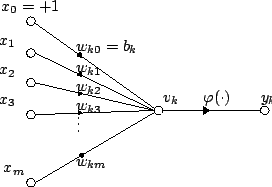
\includegraphics[width=8cm, height=6cm]{images/Artificial_neuron.png}
  \caption{Μαθηματικό μοντέλο ενός νευρώνα με bias στο $x_0 = 1$}
  \label{fig:artificial_neuron_math_model}
\end{figure}

\subsubsection{Συναρτήσεις ενεργοποίησης}

\begin{itemize}
    \item \textbf{Βηματική Συνάρτηση}: Η έξοδος αυτής της συνάρτησης είναι δυαδική και εξαρτάται από το αν η είσοδος ξεπερνά ή είναι ίση με ένα ορισμένο κατώφλι \textit{θ}. Εκτελεί μια διαίρεση του χώρου εισόδων με ένα υπερεπίπεδο. Είναι ιδιαίτερα χρήσιμη όταν εφαρμόζεται στο τελευταίο επίπεδο ενός ANN, που κάνει δυαδική συσταδοποίηση.
    \begin{CEquation}
    \begin{split}
         y = 
         \begin{cases}
         1 & \text{if}\;x\geq\theta\\
         0 & \text{if}\;x<\theta
         \end{cases}   
         \label{eq:step_function}
    \end{split}
    \end{CEquation}
    
    \item \textbf{Σιγμοειδής}: Μια μη-γραμμική συνάρτηση με παράγωγο που υπολογίζεται εύκολα, και κατ' επέκταση είναι υπολογιστικά απλή. Ένα παράδειγμα είναι η γνωστή logistic function:
    \begin{CEquation}
    \begin{split}
         y = \frac{e^x}{e^x + 1}  
         \label{eq:logistic_function}
    \end{split}
    \end{CEquation}
    
    \item \textbf{Συνάρτηση Ανόρθωσης}: Οι συναρτήσεις αυτές είναι γνωστές και ως συναρτήσεις ράμπας, και είναι το υπολογιστικό ανάλογο ενός ανορθωτή ημίσεος κύματος. Λέγονται επίσης Rectified Linear Units ή ReLU και ορίζονται ως εξής:
    \begin{CEquation}
    \begin{split}
         y = x^+ = \max{(0,x)}
         \label{eq:ReLU}
    \end{split}
    \end{CEquation}
    
\end{itemize}{}

\subsection{Οργάνωση}

Οι νευρώνες τυπικά είναι οργανωμένοι σε πολλά επίπεδα, ιδιαίτερα στην περίπτωση του deep learning. Το επίπεδο που δέχεται τα δεδομένα είναι το \textit{επίπεδο εισόδου}, ενώ το επίπεδο που δίνει το τελικό αποτέλεσμα είναι το \textit{επίπεδο εξόδου}. Μεταξύ τους μπορεί να υπάρχουν μηδέν ή περισσότερα \textit{κρυφά επίπεδα}. Τα επίπεδα μπορεί να είναι συνδεδεμένα με πολλούς τρόπους. Για παράδειγμα μπορεί να είναι \textit{πλήρως διασυνδεδεμένα}, με κάθε νευρώνα σε ένα επίπεδο να συνδέεται με όλους τους νευρώνες του επόμενου επιπέδου.

\subsubsection{Υπερπαράμετροι} \label{subsub:hyperparameters}

Μια υπερπαράμετρος είναι μια σταθερή παράμετρος της οποίας η τιμή ορίζεται πριν την εκκίνηση της διαδικασίας εκπαίδευσης. Τέτοιες παράμετροι είναι ο ρυθμός μάθησης (learning rate - LR), ή ο αριθμός των κρυφών επιπέδων.

\subsubsection{Backpropagation}

Το backpropagation είναι μια μέθοδος ρύθμισης των βαρών των συνάψεων για την διόρθωση των σφαλμάτων κατά την εκπαίδευση. Το σφάλμα πρακτικά 'μοιράζεται' σε όλες τις συνάψεις. Υπολογίζονται οι παράγωγοι των συναρτήσεων ενεργοποίησης ανάλογα με τα τωρινά βάρη, και ενημερώνονται αναλόγως με την μέθοδο βελτιστοποίησης που έχει επιλεχθεί. Σε αυτή την εργασία όλα τα μοντέλα χρησιμοποιούν τον Adam optimizer.

\subsubsection{Αρχιτεκτονικές}

Μία από τις αρχιτεκτονικές που χρησιμοποιείται σε αυτή την εργασία είναι ο πολυεπίπεδος Perceptron (Multilayered Perceptron - MLP). Η αρχιτεκτονική αυτή αποτελείται από τουλάχιστον τρία επίπεδα, ένα επίπεδο εισόδου, ένα επίπεδο εξόδου και τουλάχιστον ένα κρυφό επίπεδο, όλα πλήρως διασυνδεδεμένα μεταξύ τους. Η απλούστερη δομή (από την άποψη του αριθμού των επιπέδων) ενός MLP φαίνεται στο Σχήμα \ref{fig:multilayer-perceptron}.

\begin{figure}[h]
  \centering
  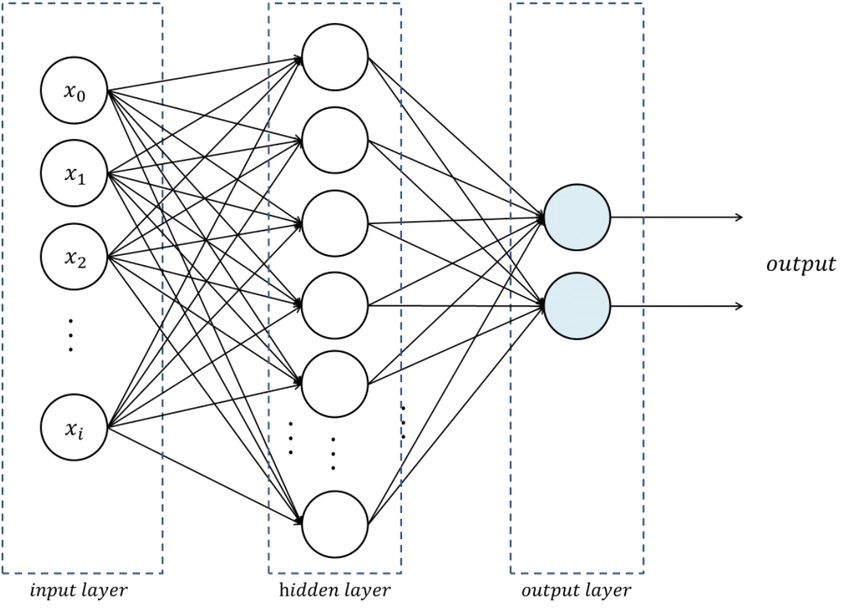
\includegraphics[width=\textwidth]{images/multilayer-perceptron.png}
  \caption{Η δομή του απλούστερου MLP.}
  \label{fig:multilayer-perceptron}
\end{figure}

Η δεύτερη αρχιτεκτονική που χρησιμοποιείται είναι αυτή των συνελικτικών δικτύων (Convolutional Neural Networks - CNNs). Η δομή αυτή είναι αρκετά πιο σύγχρονη από αυτή του MLP, και χρησιμοποιείται συχνά για την ανάλυση εικόνων και προβλήματα που αφορούν την υπολογιστική όραση. Αυστηρά, συνελικτικό δίκτυο είναι κάθε ANN που χρησιμοποιεί την πράξη της συνέλιξης. Στην πράξη, τα CNN, σε αντίθεση με τους MLP αντί να εκτολούν ένα γινόμενο πινάκων, χρησιμοποιούν συνέλιξη. Κάθε συνελικτικό επίπεδο, αποτελείται από έναν αριθμό φίλτρων που ορίζεται προτού ξεκινήσει η εκπαίδευση, όπως και οι διαστάσεις αυτών. Κάθε συνελικτικός νευρώνας επεξεργάζεται μόνο τα δεδομένα που είναι σε μια περιορισμένη υποπεριοχή της εξόδου του προηγούμενου επιπέδου. Μια τυπική δομή ενός CNN φαίνεται στο Σχήμα \ref{fig:convolutional-neural-network-architecture}. Οι λειτουργία των επιπέδων Pooling εξηγείται σε επόμενη ενότητα.

\begin{figure}[h]
  \centering
  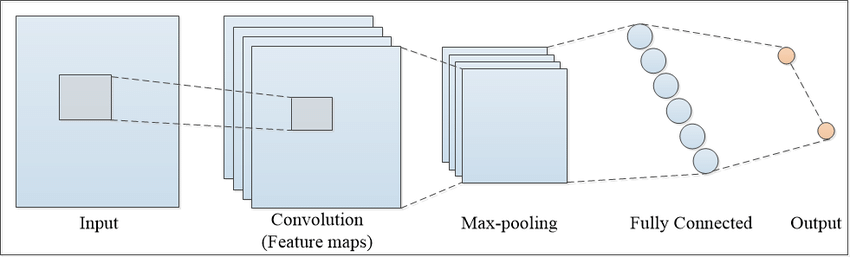
\includegraphics[width=\textwidth]{images/convolutional-neural-network-architecture-showing-a-feed-forward-pass-with-one.png}
  \caption{Η δομή ενός απλού CNN.}
  \label{fig:convolutional-neural-network-architecture}
\end{figure}
\newpage
\subsection{Συναρτήσεις Απώλειας}

Κάθε αλγόριθμος βελτιστοποίησης χρησιμοποιεί μια συνάρτηση για την \textit{αξιολόγηση} μιας πιθανής λύσης (π.χ. το σύνολο των βαρών στις συνάψεις ενός NN). Η συνάρτηση αυτή καλείται αντικειμενική συνάρτηση, και η βέλτιστη λύση είναι αυτή που ελαχιστοποιεί την αντικειμενική συνάρτηση σε προβλήματα ελαχιστοποίησης (ή το αντίθετο σε προβλήματα μεγιστοποίησης) \cite{Goodfellow2017}.

\subsubsection{Μέσο Απόλυτο Σφάλμα}
Το ΜΑΕ, είναι ένα μέτρο της διαφοράς μεταξύ δύο συνεχών μεταβλητών. Υποθέτοντας μεταβλητές Χ και Υ, οι οποίες είναι η πραγματική και η εκτιμώμενη τιμή αντίστοιχα, τότε για \textit{n} παρατηρήσεις το ΜΑΕ υπολογίζεται από την Εξίσωση \ref{eq:MAE}. Το ΜΑΕ έχει τις ίδιες μονάδες με τα δεδομένα που παρατηρούνται και πεδίο ορισμού $D = [0, +\infty)$. 

\begin{CEquation}
\begin{split}
     MAE = \frac{\sum_{i=1}^n|y_i-x_i|}{n}
     \label{eq:MAE}
\end{split}
\end{CEquation}


\subsubsection{Μέσο Τετραγωνικό Σφάλμα}
Το MSE ενός εκτιμητή, υπολογίζει τον μέσο όρο των τετραγώνων των σφαλμάτων, δηλαδή τον μέσο όρο των τετραγώνων των διαφορών της εκτιμώμενης τιμής από την πραγματική. Το MSE, είναι η δεύτερη ροπή (ως προς το 0) του σφάλματος, οπότε περιέχει τόσο την τυπική απόκλιση, δηλαδή το πόσο 'απλωμένες' είναι οι εκτιμήσεις, αλλά και  το \textit{bias}, δηλαδή το πόσο μακριά είναι η μέση εκτιμώμενη από την μέση πραγματική τιμή. Όπως η διακύμανση, έτσι και το MSE, έχει τις μονάδες των δεδομένων παρατήρησης υψωμένες στο τετράγωνο. Χρησιμοποιείται, όταν είναι ιδιαίτερα ανεπιθύμητα μεγάλα σφάλματα στον εκτιμητή, έχει πεδίο ορισμού το $D = [0, +\infty)$, και υπολογίζεται όπως φαίνεται στην εξίσωση \ref{eq:MSE}.

\begin{CEquation}
\begin{split}
     MSE = \frac{\sum_{i=1}^n|y_i-x_i|^2}{n}
     \label{eq:MSE}
\end{split}
\end{CEquation}

\subsubsection{Ρίζα Μέσου Τετραγωνικού Σφάλματος}
Το RMSE, αντιπροσωπεύει την τετραγωνική ρίζα της δεύτερης ροπής των διαφορών μεταξύ των εκτιμώμενων τιμών και των πραγματικών. Όπως και τα προαναφερθέντα μέτρα, είναι θετικά ορισμένο, με πεδίο ορισμού το $D = [0, +\infty)$. Συνδυάζει τα πλεονεκτήματα του MSE και του MAE, από την άποψη ότι 'τιμωρεί' περισσότερο τις μεγάλες αποκλίσεις από τις πραγματικές τιμές, αλλά είναι ταυτόχρονα πιο εύκολα ερμηνεύσιμο, όπως το MAE, αφού είναι και αυτό σε γραμμική κλίμακα. Υπολογίζεται όπως φαίνεται στην Εξίσωση \ref{eq:RMSE}

\begin{CEquation}
\begin{split}
     RMSE = \sqrt{\frac{\sum_{i=1}^n|y_i-x_i|^2}{n}}
     \label{eq:RMSE}
\end{split}
\end{CEquation}